\chapter{Požadavky na systém}
\textit{Tato kapitola shrnuje původní a později přidané požadavky na systém a jeho základní funkcionalitu.}

Cílem bylo vyrobit webovou aplikaci jež by uměla procházet data v RDF databázích podle předem navolenýcyh konfiguracích. Procházením se myslí postupné objevování nových uzlů grafu s pomocí již existujících uzlů. Konfigurací se pak rozumí konkrétní způsob, jak mohou být data procházena a jak jsou vizualizována. Konfigurace jsou také uloženy v RDF databázi a je tedy možné používat konfigurace z jiných datových zdrojů a naopak.

\section{Konfigurace}

V následujícím vysvětlení jsou použity tyto RDF namespacy:
\begin{table}[h] \centering
\begin{tabular}{lp{10cm}}
\toprule
\multicolumn{1}{c}{Prefix} & \multicolumn{1}{c}{IRI}                                      \\
\midrule
browser                    & \texttt{\url{https://linked.opendata.cz/ontology/knowledge-graph-browser/}} \\
dct                        & \texttt{\url{http://purl.org/dc/terms/}}
\end{tabular}
\end{table}

\subsection{Metakonfigurace} \label{pozadavky-metakonfigurace}
Metakonfigurace je skupina pro další konfigurace a metakonfigurace. Díky tomuto uživatel může procházet desíkty různých konfigurací uspořádaných do složek obdobně jak v souborovém systému na počítači. Metakonfigurace má tyto vlastnosti:

\begin{itemize}
    \item \texttt{dct:title} Název metakonfigurace \textit{(je možné zadat ve více jazycích)}
    \item \texttt{dct:description} Širší popis, co daná metakonfigurace obsahuje \textit{(je možné zadat ve více jazycích)}
    \item \texttt{browser:image} Odkaz na URL soubor s obrázkem reprezentujícím metakonfiguraci. Obrázek je pak zobrazen v aplikaci při procházení konfigurací.
    \item \texttt{browser:hasMetaconficuration} Metakonfigurace, které spadají pod tuto metakonfiguraci.
    \item \texttt{browser:hasConfiguration} Konfigurace, které spadají pod tuto metakonfiguraci. \textit{(popsáno dále)}
\end{itemize}

Metakonfigurací může být například \uv{Wikidata} nebo \uv{Otevřená data ČR}.

\subsection{Konfigurace} \label{pozadavky-konfigurace}
Konfigurací se rozumí uzel v RDF grafu který popisuje, jak by měla aplikace procházet datasety. Aktuálně může mít konfigurace tyto vlastnosti:

\begin{itemize}
    \item \texttt{dct:title} Název konfigurace \textit{(je možné zadat ve více jazycích)}
    \item \texttt{dct:description} Širší popis, čeho je možné s konfigurací dosáhnout \textit{(je možné zadat ve více jazycích)}
    \item \texttt{browser:hasVisualStyleSheet} Určuje, jak mají uzly v aplikaci vypadat. \textit{(popsáno dále)}
    \item \texttt{browser:startingNode} Doporučený uzel nebo uzly, kde začít s procházením grafu.
    \item \texttt{browser:resourceUriPattern} Regulární výraz popisující, jak by mělo vypadat IRI uzlu. Používá se v aplikaci jako nápověda uživateli, zda zadal správné IRI ještě než se pošle požadavek.
    \item \texttt{browser:hasViewSet} View sety. \textit{(popsáno dále)}
    \item \texttt{browser:autocomplete} JSON soubor se seznamem RDF uzlů podle kterých probíhá hledání. \textit{(popsáno dále)}
\end{itemize}

Příkladem konfigurace může být kupříkladu procházení slavných osobností na Wikidatech. Takováto konfigurace pak umožňuje uživateli chodit po uzlech reprezentující slavné osobnosti a dotazovat se například na filmy které natočily a knihy, které napsaly.

\subsection{ViewSet} \label{pozadavky-view-sets}
View set reprezentuje skupinu pohledů. Pravý smysl pohledů pochopí čtenář dále v textu. View set má následující vlastnosti:
\begin{itemize}
    \item \texttt{dct:title} Název view setu \textit{(je možné zadat ve více jazycích)}
    \item \texttt{browser:hasView} Pohledy které patří pod tento view set. \textit{(popsáno dále)}
    \item \texttt{browser:hasDefaultView} Výchozí pohled ze seznamu výše.
    \item \texttt{browser:hasCondition} todo
    \item \texttt{browser:hasDataset} todo
\end{itemize}

\subsection{View}
View (česky pohled) je způsob, jak můžeme pohlížet na konkrétní uzel v RDF grafu. Uzel totiž může mít obecně více vlastností současně, obdobně jako jedna osoba může být současně spisovatel, režisér a herec. V takovém případě bychom mohli mít tři různé pohledy na jeden uzel a uživatel si může vybírat, jestli ho zajímá jeho herecká, nebo spisovatelská kariéra. View má následující vlastnosti:

\begin{itemize}
    \item \texttt{dct:title} Název pohledu \textit{(je možné zadat ve více jazycích)}
    \item \texttt{dct:description} Popis pohledu \textit{(je možné zadat ve více jazycích)}
    \item \texttt{browser:hasExpansion} Odkaz na expanzi - určuje jaké uzly lze získat z daného uzlu \textit{(popsáno dále)}
    \item \texttt{browser:hasPreview} Odkaz na preview - určuje jaká data se mají získat pro ostylování konkrétního uzlu \textit{(popsáno dále)}
    \item \texttt{browser:hasDetail} Odkaz na detail - určuje která data se zobrazí v detailu konkrétního uzlu \textit{(popsáno dále)}
\end{itemize}

\subsection{Expansion} \label{pozadavky-expansion}
Expansion popisuje jak lze daný uzel expandovat, tedy jedná se o operaci kdy se stahují nové uzly jež jsou nějak příbuzné expandovanému uzlu. Expanze vrací graf, tedy expandované uzly nemusí být přímými sousedy expandovaného. Jako expanzi si můžeme představit například \uv{Zobraz všechny knihy co napsala daná osoba}. Expanze formálně partří k pohledu (view).
\begin{itemize}
    \item \texttt{dct:title} Název expanze \textit{(je možné zadat ve více jazycích, aktuálně se nepoužívá)}
    \item \texttt{browser:hasDataset} Popisuje dataset vůči kterému se dotazuje na data. \textit{(popsáno dále)}
    \item \texttt{browser:query} Popisuje SPARQL dotaz který bude spuštěn na endpointu datasetu.
\end{itemize}

\subsection{Preview} \label{pozadavky-preview}
Preview popisuje která data v rámci daného pohledu (view) popisují daný uzel. Popisem se myslí taková data, kretá mají na svědomí stylování uzlu. V aplikaci je možné mít uzly různých barev a tvarů, to právě popisuje preview. Obdobně jako expanze, preview patří ke konkrétnímu pohledu.

Preview má stejné vlastnosti jako expanze. \texttt{browser:query} v tomto případě popisuje SPARQL dotaz, který vrátí graf obsahující daný uzel a jeho literály a z těchto literálů bude sestaven preview.

Konkrétně pro preview je predikát \texttt{browser:class} považován na třídy uzlu a ty jsou nastaveny jako třídy v knihovně Cytoscape\footnote{\url{https://js.cytoscape.org/}}, která je využíváná v klientské části na krelsení grafů.

\subsection{Detail} \label{pozadavky-detail}
Detail je poslední z trojice a poskytuje dodatečné informace k uzlu. Může se jednat o literály které nemá smysl v dané konfiguraci vykreslit do grafu jako uzly, proto budou zobrazeny v bočním panelu aplikace.

Detail má stejné vlastnosti včetně \texttt{browser:query} jako preview.

\subsection{Dataset}
Dataset popisuje SPARQL endpoint vůči kterému probíhá dotazování na data.

\begin{itemize}
    \item \texttt{dct:title} Název datasetu \textit{(aktuálně se nepoužívá)}
    \item \texttt{void:sparqlEndpoint} URL adresa SPARQL endpointu na kterou se posílají SPARQL dotazy
    \item \texttt{browser:accept} todo
\end{itemize}

\subsection{Visual style sheet} \label{pozadavky-visual-style-sheet}
Popisuje jakž styl mají mít uzly v dané konfiguraci. Popis je založen na datech pocházejících právě z \textbf{preview}. Forma zápisu stylů aktuálně odpovídá stylům jaké používá knihovna Cytoscape.

Visual style sheet má pouze jednu vlastnosti

\begin{itemize}
    \item \texttt{browser:hasVisualStyle} Jedno pravidlo jak se má provést stylování, odkazuje na \textbf{Visual style}.
\end{itemize}

\subsubsection{Visual style}
Visual style má pak:

\begin{itemize}
    \item \texttt{browser:hasSelector} Selector pro Cytoscape knihovnu, jež vybírá na které uzly nebo hrany daný styl bude aplikován.
    \item \texttt{browser:*} Jednotlivá pravidla jak má být daný uzel nebo hrana ostylována. Používají se přesně ty názvy, které používá knihovna Cytoscape, kupříkladu \texttt{browser:border-width} nebo \texttt{browser:background-color}.
\end{itemize}

\section{Aplikace}

Bylo zamýšleno, že klientská aplikace bude komunikovat se serverovou částí, která bude stahovat data z různých datových zdrojů a výsledky posílat zpět klientské aplikaci. Ta v případě potřeby bude stahovat přímo z internetu obrázky, pokud na ně uzly odkazují. Idea rozdělení klienta a serveru byla v tom, že v budoucnu může být na serveru implementováno chachování, aby aplikace byla plynulejší a neprobíhalo zatěžování datových zdrojů.\footnote{Při příliš rychlém stahování z Wikidat lze bohužel snadno dostat IP ban, tedy alespoň pro Wikipedii je cachování nezbytné.}

Chachování aktuálně implementováno ještě není, server je tedy kompletně bezestavový.

\begin{figure}[h]
    \centering
    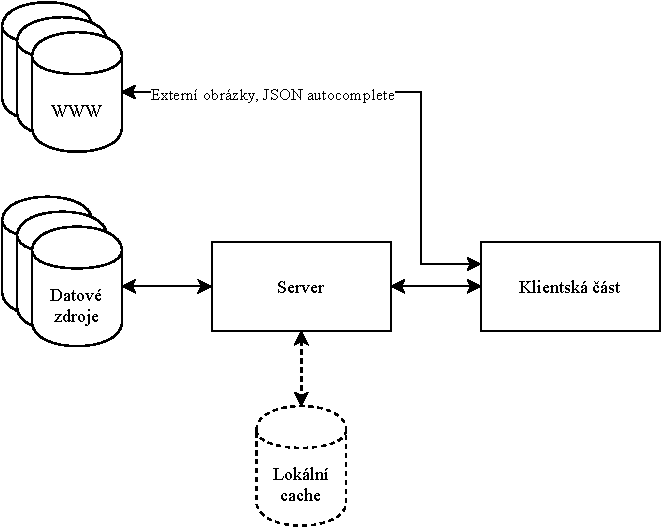
\includegraphics[width=0.75\textwidth]{media/communication.pdf}
    \caption{Komunikace mezi klientem, serverem a datovými zdroji. Cachování na serveru ještě implemontováno není.}
\end{figure}

\subsection{Server}
Převážná část serveru byla napsána mým vedoucím a sloužila jako forma specifikace na klientskou část. Server bude podrobněji rozebrán v další kapitole.

\subsection{Klient}
Požadavkem bylo vyrobit webovou aplikaci schopnou komunikovat se serverem a uživateli vizuálně zobrazovat uzly a hrany na obrazovce. Mezi původními požadavky na software bylo (požadavky jsou zkráceny):

\begin{enumerate}[topsep=0pt,itemsep=-1ex,partopsep=1ex,parsep=1ex]
\item Uživatel je schopen vybrat IRI konfigurace.
\item Uživatel je schopen vybrat IRI stylesheetu podle kterého budou obarveny a jinak zvýrazněny uzly.
\item Uživatel je schopen přidat uzel na základě jeho IRI a zobrazit si k němu detail.
\item Pokud uživatel klikne na uzel, zobrazí se mu nabídka s detailem a možností další expanze.
\item \textit{sjednoceno do 4}
\item Uživatel může uzel skrýt. V menu je možnost zobrazit skryté uzly.
\item Dvojklikem na uzel se provede expanze podle aktuálního pohledu. Tu je možné provést také pomocí požadavku 4.
\item Uzly je možné filtrovat podle grafových vlastností.
\item Uzly je možné filtrovat podle sémantických vlastností.
\item Uživatelské rozhraní je multijazyčné.
\item Graf je možné uložit do souboru a poté jej ze souboru obnovit.
\item Uživatel může uzel z grafu smazat.
\item Uživatel může přidávat uzly pomocí autocomplete z před připraveného JSON souboru.
\end{enumerate}

Časem byly do aplikace doplněné další požadavky jako
\begin{itemize}[topsep=0pt,itemsep=-1ex,partopsep=1ex,parsep=1ex]
\item Volba různých layoutů.
\item Uzly mohou být seskupovány do skupin.
\item Podpora metakonfigurací.
\end{itemize}